\section{Auswertung}
\label{sec:Auswertung}
\subsection{Messung des Schwellenstroms}
In dem Versuchsteil wurde ein Schwellenstrom von $I_S = \SI{65.2}{\milli\ampere}$ bestimmt. Ein Foto der Detektorkarte direkt vor und nach erreichen der Lasergranulation sind in Abbildung \ref{pic:vschw} und \ref{pic:nschw}
zu finden.
\begin{figure}
    \centering
    \includegraphics[width = 0.78\textwidth]{pictures/vschw.png}
    \caption{Kurz vor erreichen des Schwellenstroms}
    \label{pic:vschw}
\end{figure}
\begin{figure}
    \centering
    \includegraphics[width = 0.78\textwidth]{pictures/nschwelle.png}
    \caption{Lasergranulation beim erreichen des Schwellenstroms}
    \label{pic:nschw}
\end{figure}

\subsection{Fluoreszenz und Transmissionsspektrum}
Bei einem Strom von $I = \SI{65.2}{\milli\ampere}$ ist ein Foto der Rubidiumfluoreszenz in Abbildung \ref{pic:flu} zu sehen.
Das Transmissionsspektrum ist in Abbildung \ref{pic:ab} zu sehen und wurde bei dem selben Strom aufgenommen.
Mit Abbildung \ref{pic:energie} lassen sich die Transmissionslinien von links nach
rechts mit den 85a, 87a, 85b, 87b linien identifizieren.
\begin{figure}
    \centering
    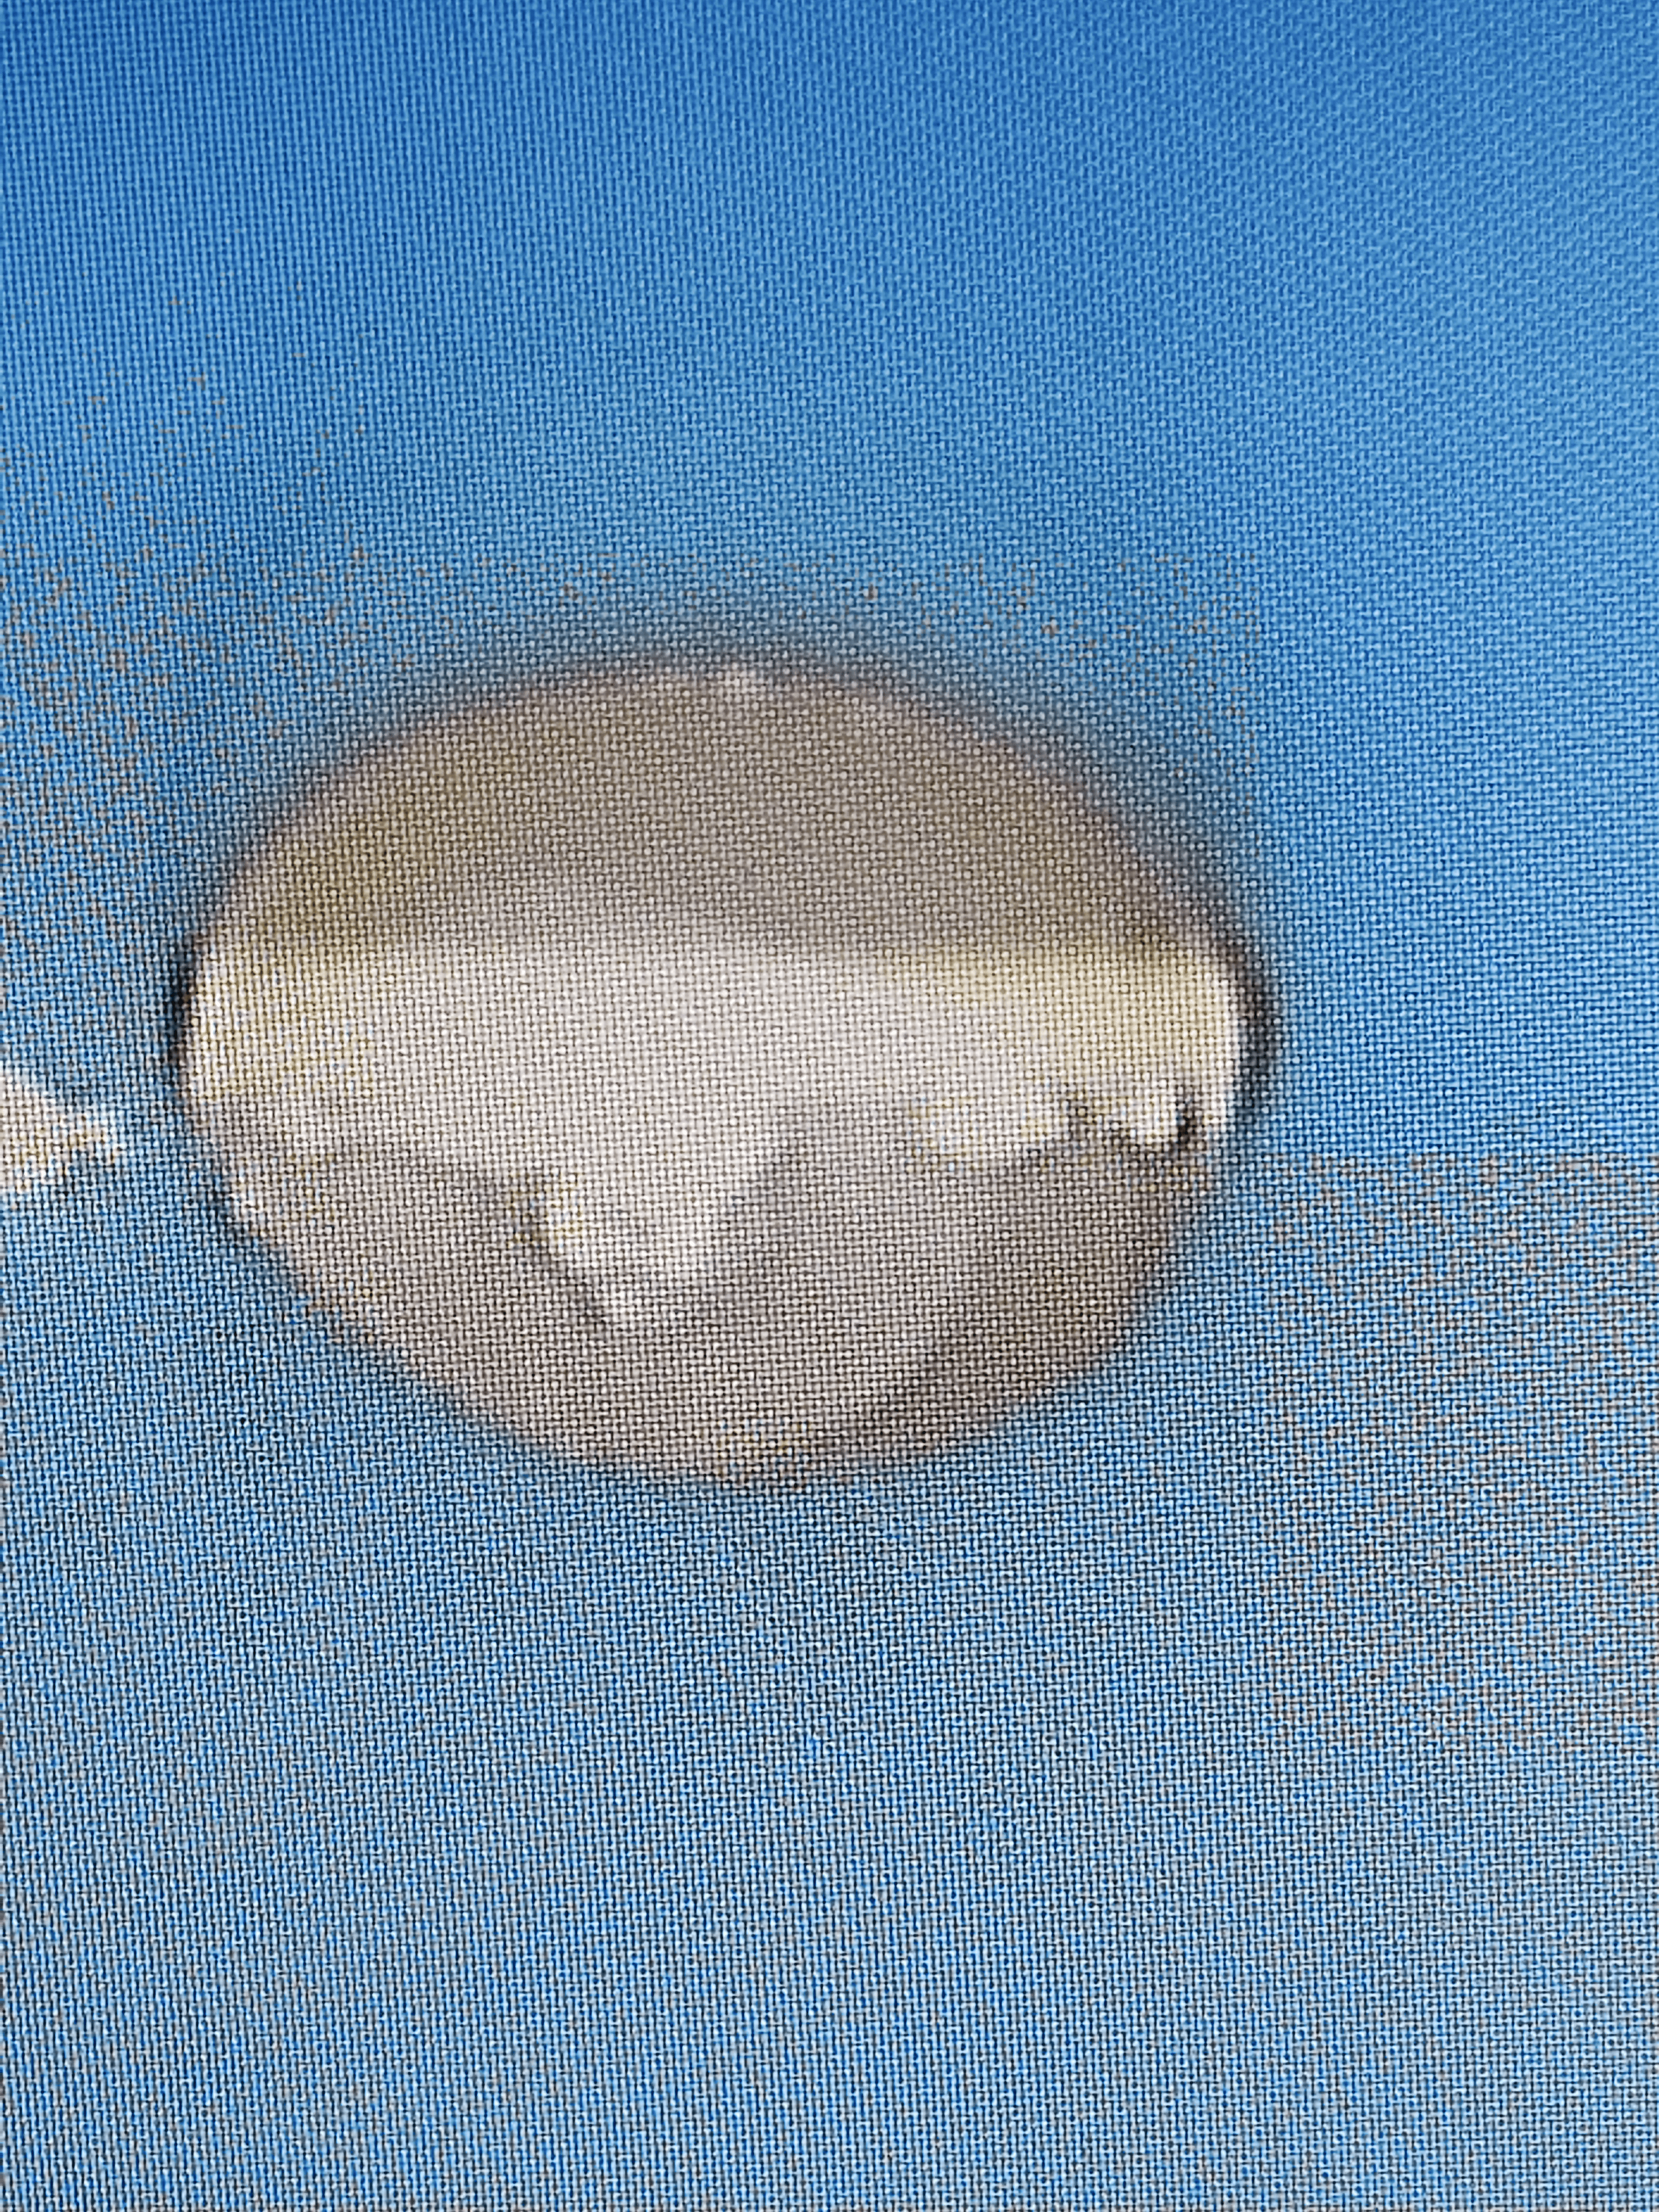
\includegraphics[width = 0.78\textwidth]{pictures/fluo.png}
    \caption{Beobachtete Fluoreszenz des Rubidiums}
    \label{pic:flu}
\end{figure}
\begin{figure}
    \centering
    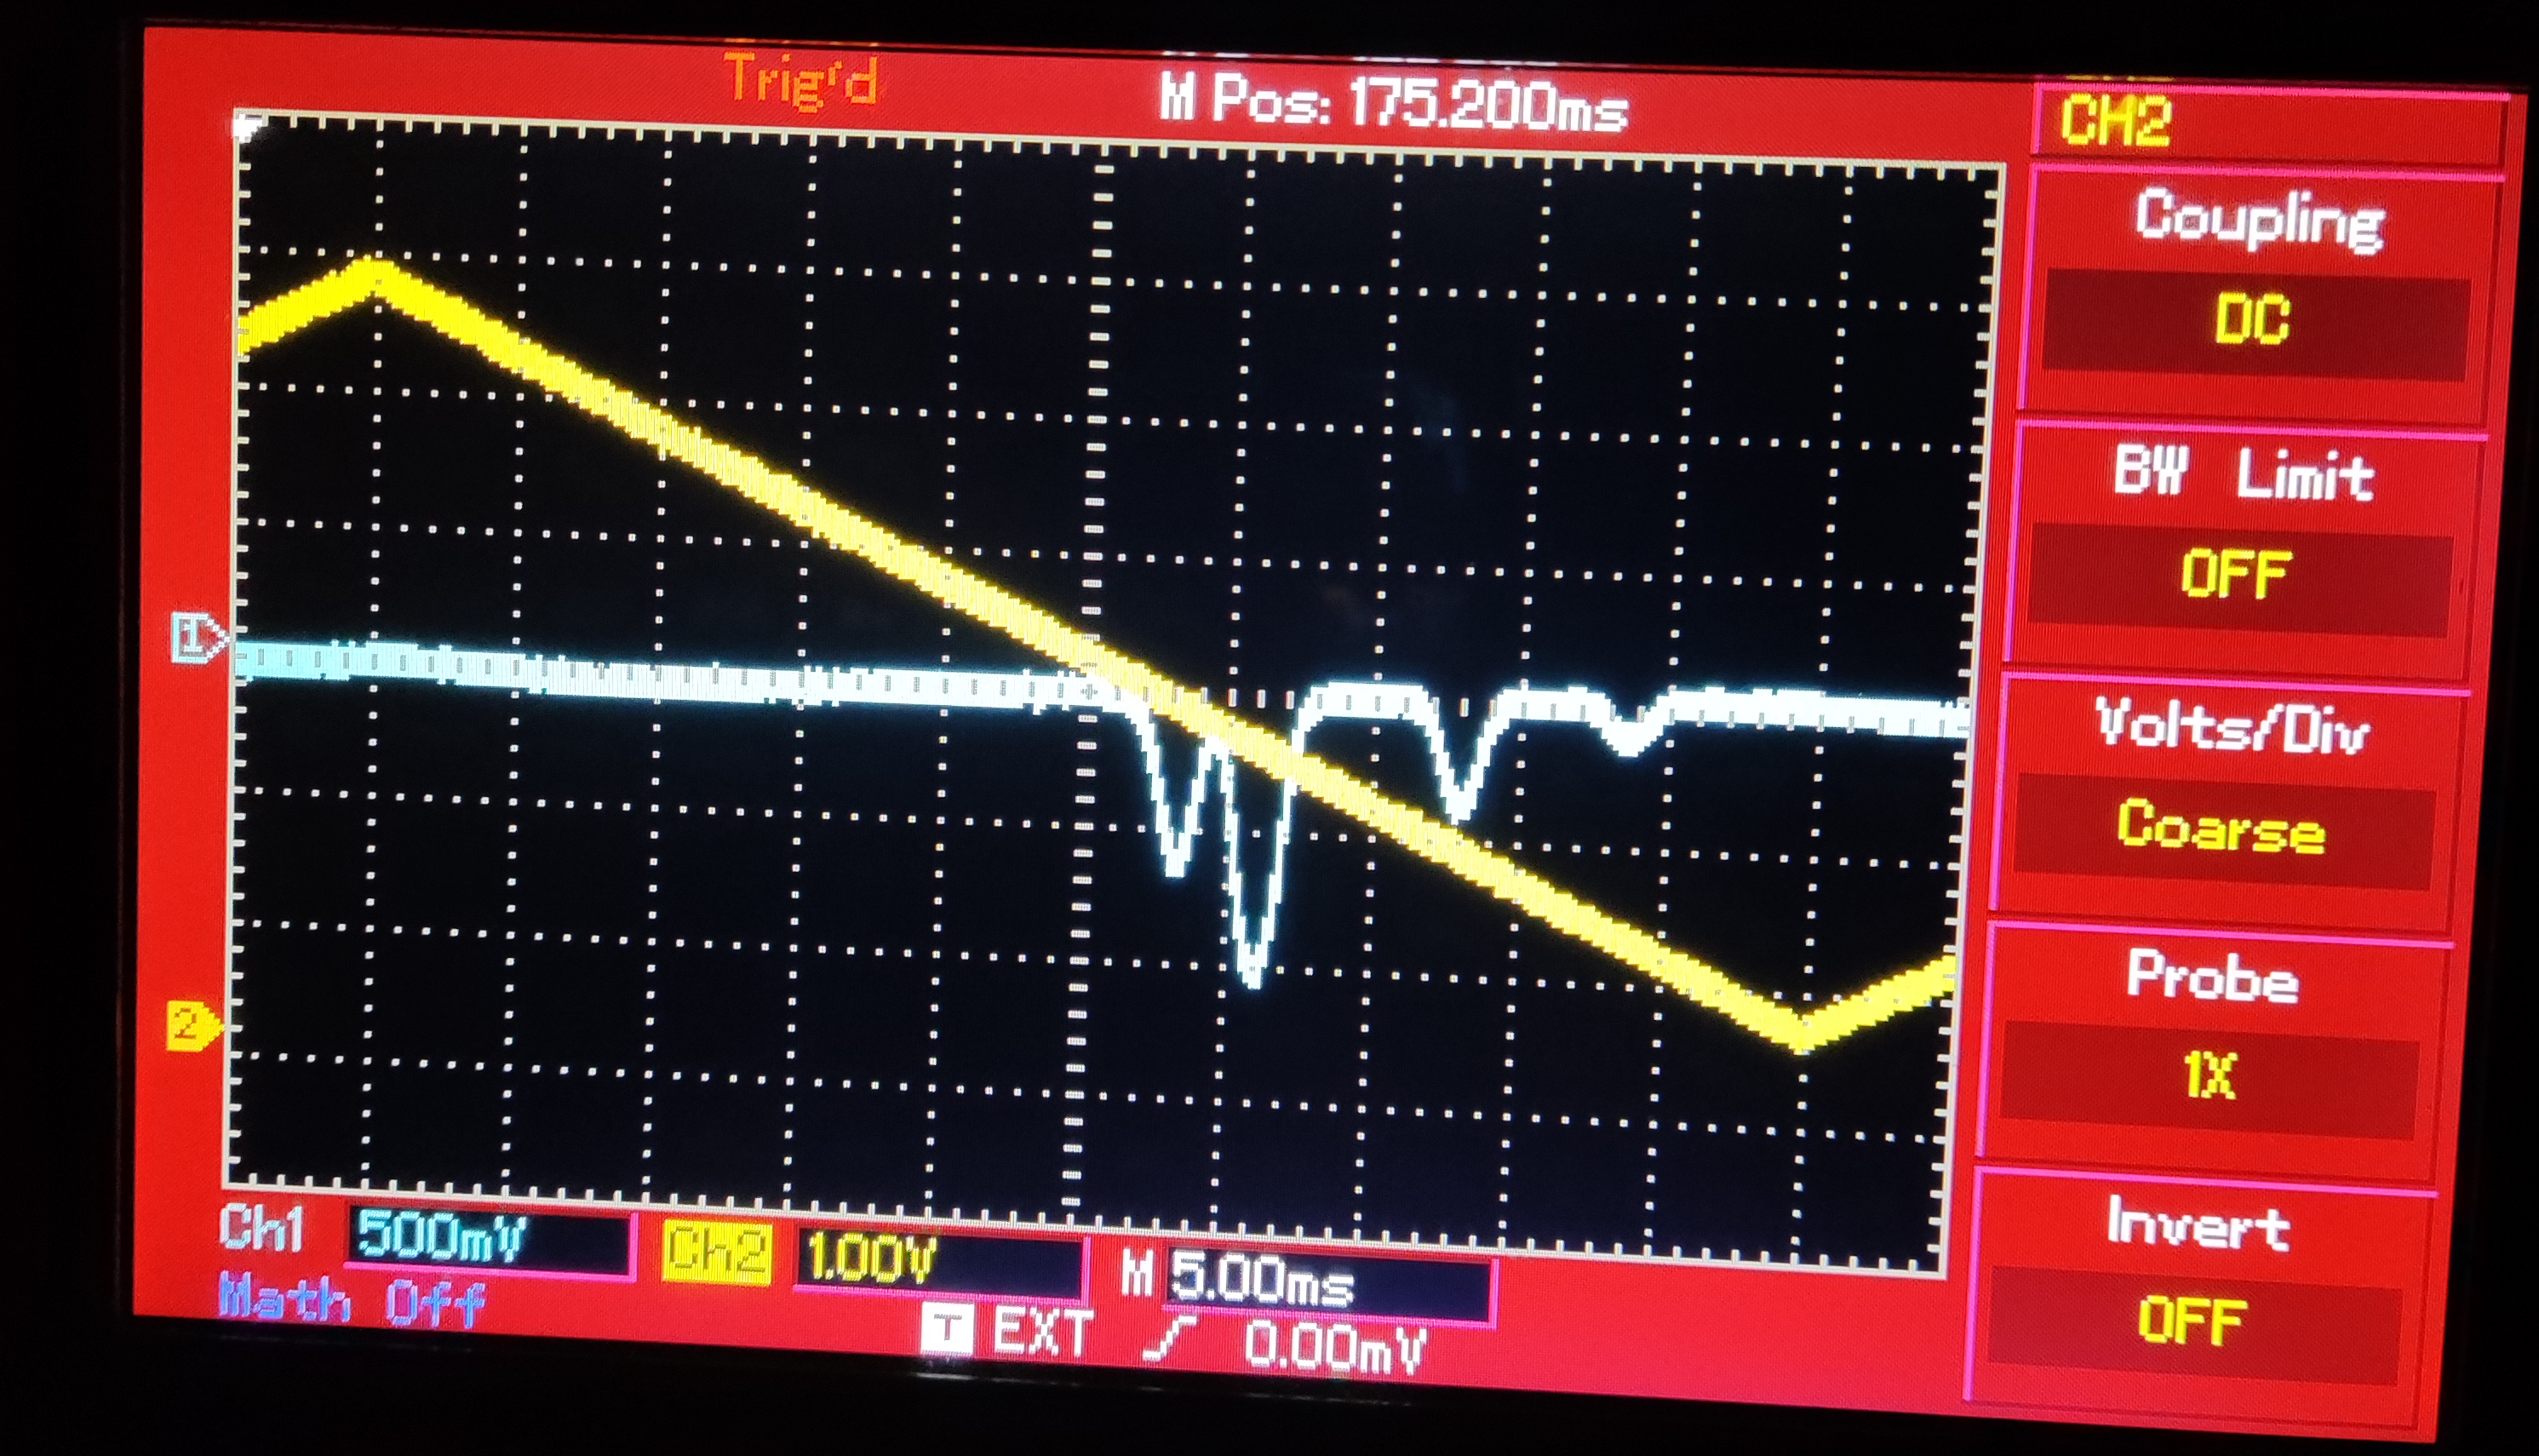
\includegraphics[width = 0.78\textwidth]{pictures/abso.png}
    \caption{Transmissionsspektrum ohne Untergrund}
    \label{pic:ab}
\end{figure}